

\section{Introduction}
\label{sec:corpusCreation.introduction}



%\todo{ Computational social science runs on twitter data.
%7.7M google scholar results for twitter, with over 140k in just 2022.
%How many of these studies query for a hashtag or keyword to build a corpus?
%How many would benefit from training a classifier to filter out irrelevant tweets?}

The wide-spread availability of social media data
has resulted in an explosion of social science studies
as researchers adjust
from data scarcity
to abundance
in the internet age~\cite{lazer2009computational,lazer2021meaningful}.
The potential for large scale digitized text to
help understand human behavior seems boundless.
Researchers have attempted to broadly quantify language use of societies over time, 
whether with digitized books
or with large scale social media datasets~\cite{michel2011quantitative,alshaabi2021storywrangler}.
However, for more targeted studies using social media data, researchers need a principled way to define the boundaries of their corpus~\cite{shugars2021pandemics}.

Analysis of social media data promises to supplement
traditional polling methods
by allowing for
rapid, near real-time measurements
of public opinion,
and allowing for historical studies of public language \cite{oconnor2010, cody2015climate, cody2016, wu2023}.
Polling remains the gold standard
for measuring public opinion where precision matters,
such as predicting the outcomes of elections 
\todo{Examples of public opinion measurements, (BLM, covid, climate, war, marketing, etc)}.

When researchers characterize online discourse around a specific topic, a few approaches are available.
Each comes with trade-offs, both in researchers' time as well as the resulting precision and recall of the corpus.

Keyword filters can be an effective strategy for corpus curation, for example by querying relevant hashtags 
which signal an author's intent to label their post as belonging to a topic.
Keywords can also be used to match relevant posts with high precision, but often low recall.
Hashtag based queries have been used by researchers
to construct focused corpora of tweets ranging from sports and music~\cite{blaszka2012worldseries,choi2014south},
to natural disasters, political activism, and
protests~\cite{steinert2015online,lotan2011arab,freelon2016beyond,jackson2020hashtagactivism,gallagher2019reclaiming,gallagher2018divergent,gorodnichenko2021social,arnold2021hurricanes}.

Alternatively, researchers can query for posts with an expansive set of keywords
to increase recall at the expense of precision. 
Researchers looking to expand this set of keywords can do so algorithmically,
or by querying individuals with domain expertise, or via a combination of the two.
Broad expert crafted keyword lists have been used to study
social responses to the COVID-19 pandemic~\cite{shugars2021pandemics,chen2020tracking,green2020elusive,twitter_2020}%\todo{Add more examples here?}.
Other researchers have algorithmically generated lists of keywords, e.g., using Term Frequency - Inverse Document Frequency (TF-IDF)~\cite{aizawa2003information} and word embeddings~\cite{marujo2015automatic} or
by comparing the distribution of words in a corpus of interest to a reference corpus
and selecting words with high rank-divergence contributions~\cite{dodds2020allotaxonometry,alshaabi2021world,minot2022distinguishing,alajajian2015,stupinski2022quantifying}. 
Regardless of the algorithm, continued expansion beyond the most relevant keyword necessarily reduces precision. 
Researchers can further refine the set of relevant keywords to balance precision and recall,
or add complexity to their queries with negation or Boolean operators to require multiple keywords.

% central pitch
While some social media datasets can be sufficiently curated
with simple heuristics
or rules-based classifiers,
others could benefit from an alternative paradigm.
We argue for a two step pre-processing pipeline
that combines broad,
high recall keyword queries
with fine-tuned,
transformer-based classifiers
to increase precision.
This approach can trade the labor costs associated with building rules-based filters, 
for the cost of labeling social media data for few-shot learning~\cite{wang2020generalizing}, while still achieving high precision.

% history of language models
The tools available for text classification have improved significantly over the past decade.
Since the introduction of Word2Vec in 2013 and GloVe in 2014,
the natural language processing community has had access to high quality, global word embeddings~\cite{mikolov2013efficient,pennington2014glove}.
These embeddings are trained vector representations of words from given a corpus of text,
enabling word comparisons with distance metrics.
However, global embeddings average the representations of words,
making them unsuitable for document classification
where key terms have multiple meanings.
The development of large pre-trained language models
enabled high performance on downstream tasks with relatively little additional computational cost to fine-tune~\cite{devlin2018bert,liu2019roberta}.
Such models provide contextual, rather than global, word embeddings. 

%incremental improvement in language models
Since 2019, pre-trained language models have become less resource intensive while improving performance.
Knowledge distillation has enabled models like DistilBert and MiniLM, 
which retain the performance of full sized models while requiring significantly less memory
and performing inference faster~\cite{sanh2019distilbert,wang2020minilm}. 
Smaller, faster models enable researchers with limited resources to adopt these tools for NLP tasks, requiring only a laptop for state-of-the-art performance.
Improved pre-training, introduced with MPNet,
combines the benefits of masked language modeling (MLM)
and permuted language modeling (PLM),
better utilizing available token and position information~\cite{song2020mpnet}.  

Transformer-based language models provide state of the art performance on natural language processing tasks,
they can be difficult to understand and visualize. 
Using twin and triplet network structures,
pre-trained models can be trained to generate 
semantically meaningful sentence embeddings that can be compared using cosign distances~\cite{reimers-2019-sentence-bert}.

Text classification still remains a challenging task. Existing models are less successful with longer texts~\cite{gao2021limitations}. And text classification with a large number of classes remains challenging~\cite{chang2020taming}. 
However, for the specific task of classifying tweets~\cite{antypas2022twitter}, 
short texts limited to 280 characters, 
as relevant or not relevant to a specific topic, 
an instance of binary classification,
we feel existing models are sufficiently performant.
Sophisticated, pre-trained language models are readily accessible to researchers from Hugging Face~\cite{wolf2020transformers}
and can be easily fine-tuned with a limited amount of labeled data~\cite{yan2018few,wang2020generalizing}.


%The two recent improvements in language models, 
%their improved contextual performance and reduced model sizes, enabled by knowledge dis


As a case study we examine online language around emission-free energy technologies. 
In democratic societies the social perception of technologies
affects the willingness of governments
to extend subsidies,
expedite permitting,
or regulate competing energy sources, 
ultimately effecting the energy mix of the grid. \todo{cites from Kim et al}
Quantifying public attitudes is useful for policy makers to be responsive to public preferences
and for science communicators to respond when public opinion doesn't reflect expert consensus.

To quantify public perceptions of energy on social media sites,
researchers have use a variety of methods to curate tweet corpora. 
This could be as simple as querying for a single hashtag; Jain et. al. choose `\#RenewableEnergy'  to generate a corpus for a renewable energy classification study~\cite{jain2019sentiment}.
Zhang et. al. query for tweets containing a list of hashtags,
before quantifying overall attention trends and sentiment by energy source~\cite{zhang2022perceptions}.
Li et. al. use a two-phase approach, querying for relevant hashtags, before filtering non-relevant tweets with keywords, such as those containing both `\#solar' and `eclipse', with filter keywords built on a trial-and-error approach~\cite{li2019beyondBigData}
Alternatively, Kim et. al. use keyword phrases,
such as `solar energy' and `solar panel', to search for relevant tweets,
before using RoBERTa to classify sentiment~\cite{kim2021public}.
On Reddit Kim et. al. study renewable energy discourse by collecting all messages from a particular subreddit,
a page devoted to a topic,
before analyzing a word co-occurrence network~\cite{kim2020exploring}.

Published studies use a wide range of corpus curation techniques
and provide varying levels of justification for each choice.
Although we focus on the topic of renewable energy, we hope our methods are broadly applicable
to any text-based social media dataset.

We structure the remainder of this paper as follows. In Methods and Data present a description of our dataset and discuss the task of relevance classification as it relates to corpus curation. In Results, we present case studies for the keywords \anchor{solar}, \anchor{wind}, and \anchor{nuclear}. We examine the ambient sentiment timeseries for each corpus, and compare measurements between the unfiltered, relevant and non-relevant text. To show the differences in language between these corpora, we present sentiment shift plots~\cite{gallagher2021generalized} and allotaxonographs~\cite{dodds2020allotaxonometry}. Finally, we present concluding remarks.

\section{Methods and Data}
\label{sec:corpusCreation.methods}



We explore the performance of text classifiers
powered by contextual sentence embeddings
for social media corpus curation
through a selection of case studies related to clean energy. 




\subsection{Description of data sets}
\label{sec:corpusCreation.data}

In this study we examine ambient tweet datasets,
collections of tweets that are anchored by a single keyword or set of keywords. 
From Twitter's Decahose API,
a random 10\% sample of all public tweets,
we select tweets containing a user-provided locations~\cite{twitterDecahose}. 
We extracted these locations from a free text location field in each user's bio,
if the text matched a valid 
\texttt{`city, state'} string in the United States~\cite{gray2018english, linnell2021sleep}.
From this selection,
we query for tweets that both contain keywords of choice and are classified as English by FastText~\cite{joulin2017bag}.
We define the results of this query as the unfiltered ambient corpus.

To illustrate the utility of our methodology,
we chose three keywords related to non-fossil fuel energy generating technologies, \texttt{`wind'}, \texttt{`solar'}, and \texttt{`nuclear'}. 
Over the study period from 2016 to 2022,
these keywords matched 3.43M, 1.39M, and 1.29M tweets in our subsample, respectively.
While the terms of service with Twitter do not allow us to publish raw tweets,
we provide relevant tweet IDs for rehydration. 
\todo{Add tweet\_id extractor to git repo.}


\subsection{Sentence embeddings}
To better visualize the results of our classification algorithms, we chose pre-trained language models which had been fine-tuned to perform sentence embeddings. We found that the performance of classification was not noticeably impacted by using models trained 


\subsection{Relevance classification}
Our task of interest is classifying if a post, 
in its entirely,
is relevant to the researcher's chosen topic of interest. 
Conceptually, this task is related to semantic textual similarity (STS), 
for which sentence embeddings have achieved state of the art performance. 
Rather than finding nearest neighbors in a semantic space,
we are training a classifier to partition the semantic space into relevant and not relevant regions.

For training we hand-label a random sample of 1000 matching tweets
for each keyword
as either `relevant' (R)  or `not relevant' (NR) to energy production. 
We've made tweet IDs and corresponding labels available for both the training data 
as well as predicted labels for the full data set.
\todo{add this}


We fine-tune seven models for comparison, based on pre-trained contextual sentence embeddings~\cite{song2020mpnet, wang2020minilm, }.

We list the performance of the models in Table~\ref{tab:F1-scores}.

\todo{Add some more model F1 scores, maybe a for L6, and for Glove if you can do it with Hugging Face, + for just normal BERT and else go edit?}


\begin{table}[t]
    \begin{tabular}{  l p{1.1cm} p{4.55cm} }
        \toprule
        \textbf{Keyword} & \textbf{Class}     
        & \textbf{Example Tweet}   \\\midrule
    Solar & (R)
            &  The decreasing costs of solar and batteries mean a sustainable future is closer than we think.  \\ \cmidrule(lr){2-3} 
        & (NR)      
            & Looks like there's a solar eclipse down here. The space nerds bought all the hotel rooms.    \\\midrule
    Wind & (R)      
            & At this time of year wind makes up only a fraction of the state's energy generation mix.  \\ \cmidrule(lr){2-3} 
        & (NR)      
            & His mom caught wind of what they were up to and shut down their plans pretty quickly. \\\midrule
    Nuclear & (R)
            & Nuclear activists are questioning \#MAYankee's accelerated decommissioning plan. \\ \cmidrule(lr){2-3} 
        &  (NR)      
            & The global nuclear arsenal stands around 10,000 warheads, down from 70,000 at the peak of the Cold War. \\
        \bottomrule
    \end{tabular}
    \caption{Paraphrased example tweets for relevant (R) and not relevant (NR) examples in each case study. To label the training data, we defined relevant tweets as those which are related to the topic of electricity generation or clean energy. Not relevant tweets contained the keyword, but were wholly or primarily unrelated.
    }
    \label{tab:example_tweets}
\end{table}


\begin{table}[t]
\begin{tabular}{lllll}
\toprule
   & \anchor{solar} & \anchor{wind} & \anchor{nuclear} \\
     \cmidrule(lr){2-4} 
   \% Relevant  & 43.7\% & 4.7\% & 16.0\% \\
   \midrule
    F1 - MPNet                  & 0.951     & \textbf{0.903}  & 0.860  \\
    F1 - MiniLM-L12             & 0.933     & 0.839   & 0.879  \\
    F1 - MiniLM-L6              & 0.949     &  0.828  & 0.857   \\
    F1 - DistilRoberta          & \textbf{0.956}  &  \textbf{0.903}  & 0.857  \\
    F1 - paraphrase-MiniLM-L6   & 0.943     &  0.800  & 0.826  \\
    F1 - paraphrase-MiniLM-L3   & 0.918     &  0.714  & 0.814  \\
    F1 - distiluse-multilingual & 0.929     &  0.759  & \textbf{0.912}  \\

  \bottomrule
\end{tabular}
\caption{\texttt{Summary statistics} for each of the three case studies.
First, we report the proportion of human labeled tweets
that are labeled relevant to clean energy from our thousand tweet subsample.
The \anchor{solar} corpus was most evenly split,
while the \anchor{wind} corpus was the most imbalanced. 
Second, we report the F1 evaluation score for fine-tuned
text classifiers trained on our labeled data.
The model performance doesn't necessarily degrade
for corpora with a small proportion of relevant documents, like for \anchor{wind}.} 
\label{tab:F1-scores}
\end{table}



\subsection{Corpus Comparison}

\todo{Corpus comparison}
To quantify the differences between the filtered, unfiltered text








% Figure 1
\begin{figure*}
  \centerfloat	
        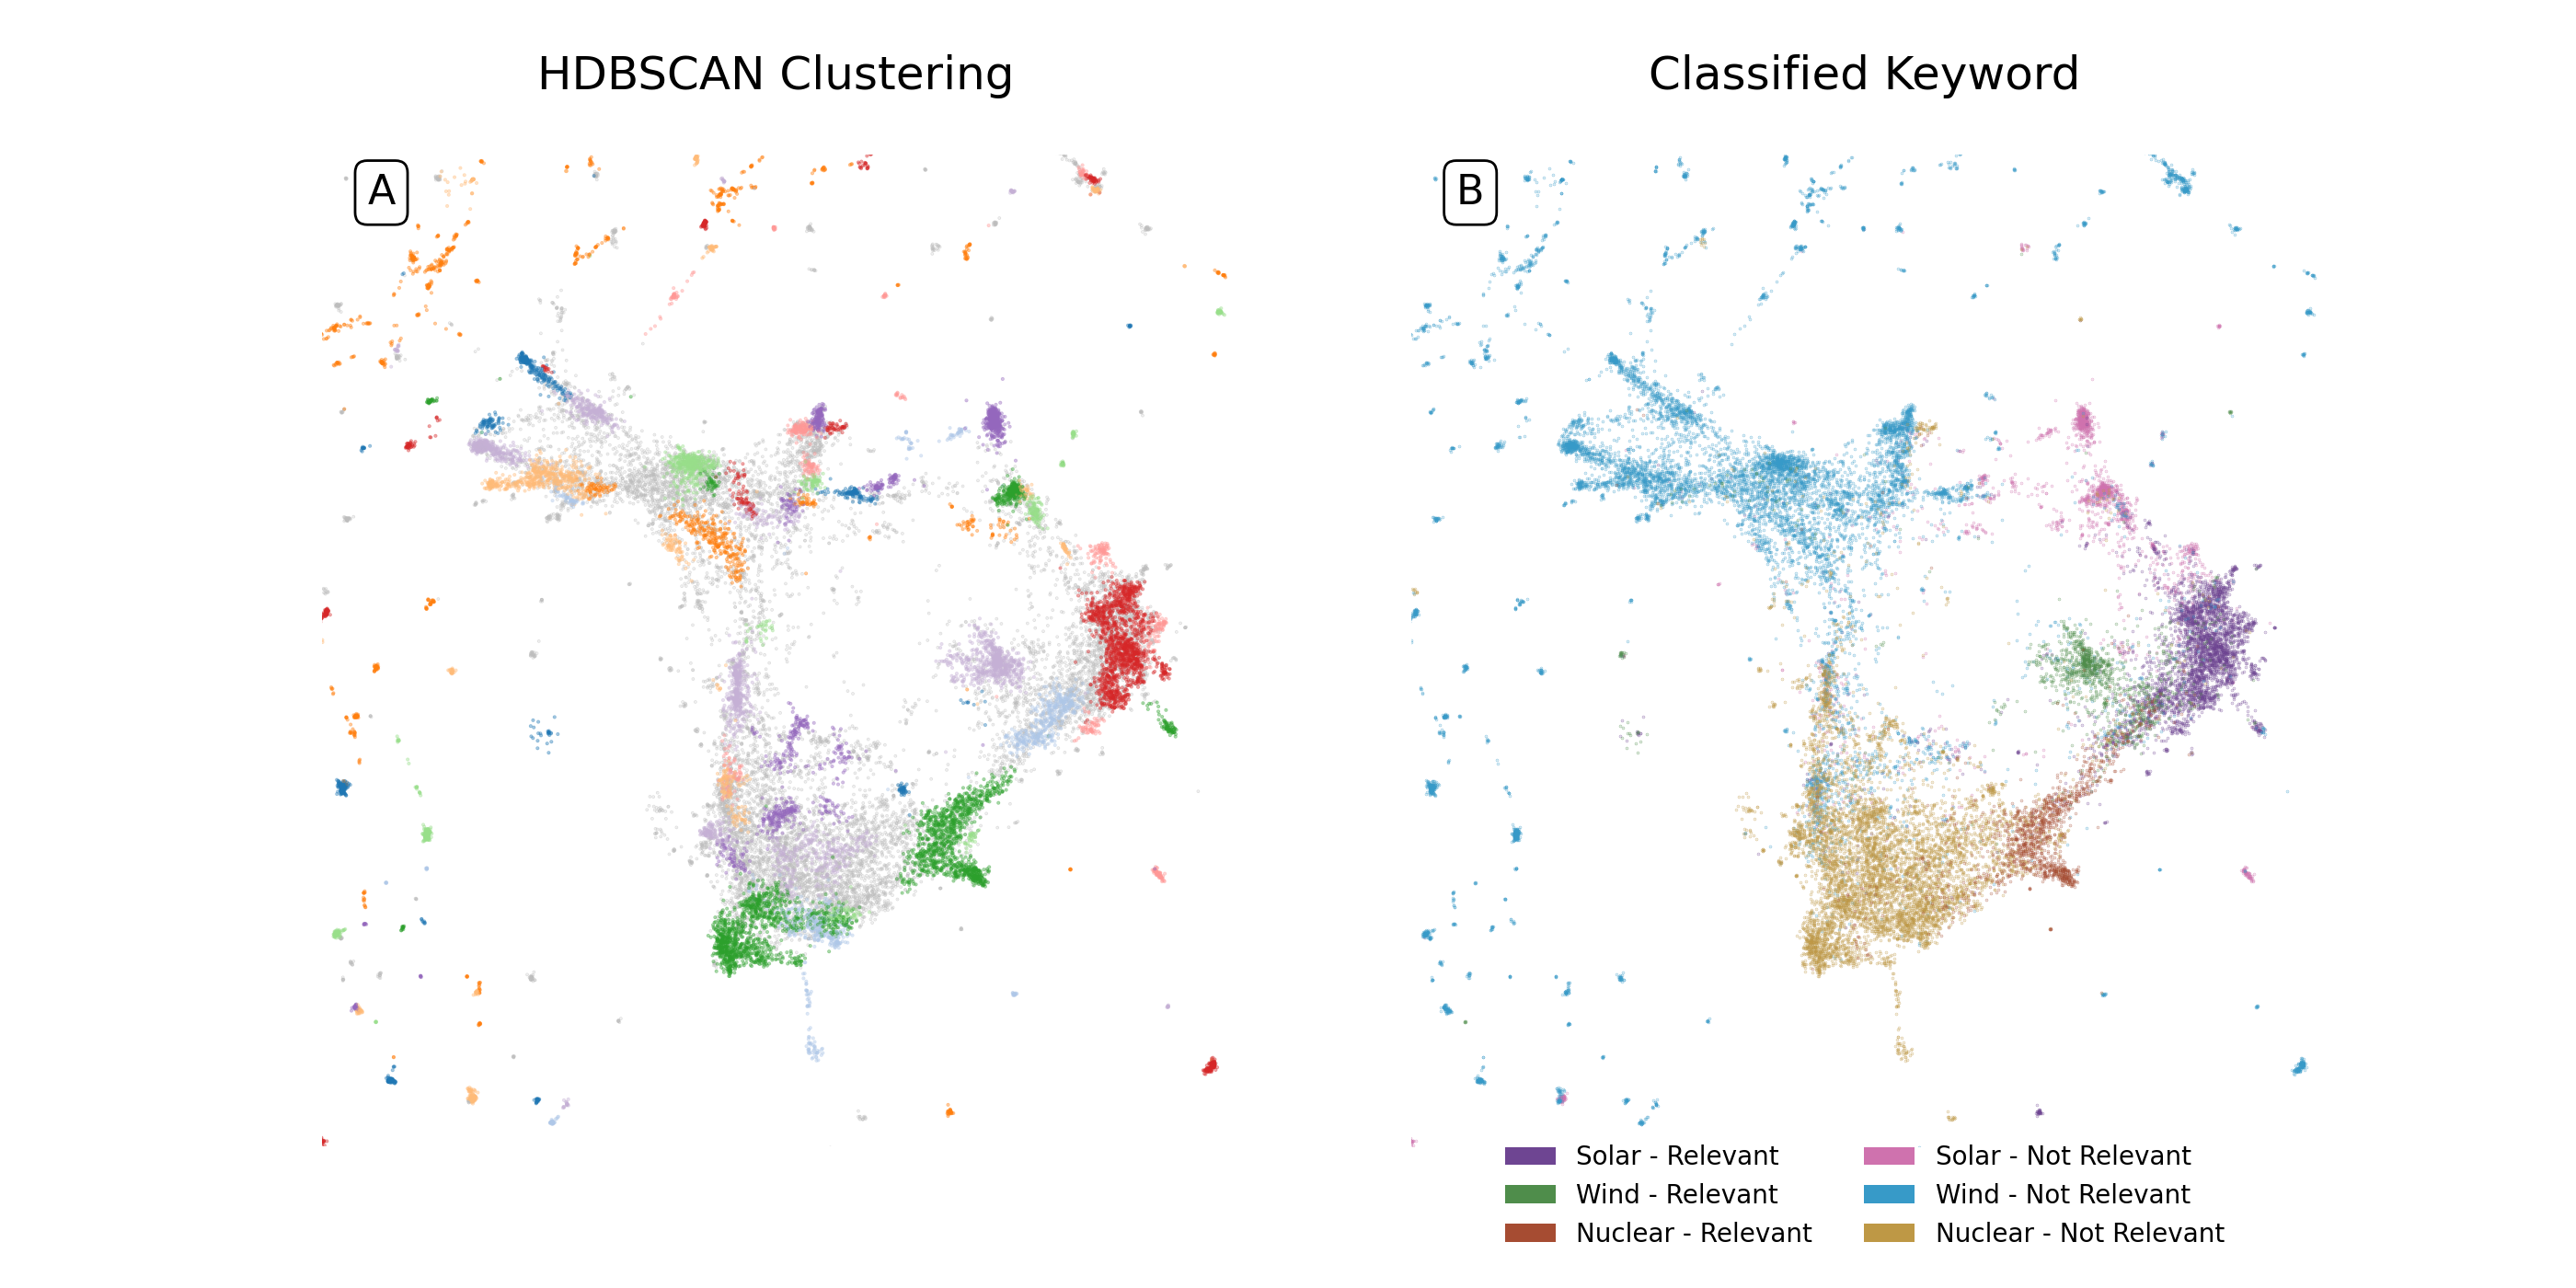
\includegraphics[width=2.8\columnwidth]{figures/combined_labeled_embedding_horizontal.png} 
  \caption{\textbf{Embedded tweet distribution plot} for the combined datasets.
  Using a pre-trained model for semantically meaningful sentence embeddings based on MPNet, we plot the distribution of tweets within this semantic space.
  In both plots, points are tweets projected into 2D using UMAP for dimensionality reduction~\cite{mcinnes2018umap}.
  In panel A, we perform density based, hierarchical clustering using HDBSCAN and color by cluster.
  In panel B, we color by both the keyword used to query and the classification as relevant or not relevant to the topic of clean energy. 
  Relevant tweets containing the keywords \anchor{wind}, \anchor{solar}, and, to a lesser extent, \anchor{nuclear} are relatively close together on the right in the embeddings, while not relevant tweets are more dispersed.} 
    \label{fig:combined_embeddings}
\end{figure*}


\todo{Expand on fine-tuning and classification procedure.}






\section{Results}
\label{sec:corpusCreation.results}

We first examine our corpus within a semantically meaningful sentence embedding, shown in Fig.~\ref{fig:combined_embeddings}. 
For each tweet
we compute embeddings using \texttt{all-mpnet-base-v2},
a high performing, general-purpose sentence embedding model based on MPNet. It is pre-trained to minimize cosign distance between a corpus of 1 billion paired texts and accessed using the sentence transformers python package~\cite{reimers-2019-sentence-bert}.
We include embeddings all three corpora, anchored by the keywords \anchor{solar}, \anchor{wind}, and \anchor{nuclear}, and project into two dimensions for visualization using Uniform Manifold Approximation and Projection (UMAP) for dimensionality reduction~\cite{mcinnes2018umap}. 
In the 2D projection, semantic distances between are distorted.
Local relationships are preserved, but global position and structure is not. 

In panel A, we perform unsupervised clustering using HDBSCAN and color by cluster~\cite{mcinnes2017hdbscan}. \todo{Add some extra here}

In panel B, we show the results of our three supervised text classifiers, based on MPNet and fine-tuned on a dataset of 1000 labeled tweets for each keyword.
The local positioning of tweets within the embedding reflects similarity in the sentence embedding space.
Tweets classified as relevant to clean energy technologies are clustered on the right-hand side, and overlap where they are mentioned together.
For paraphrased example tweets with each classification, refer to Table \ref{tab:example_tweets}.

On the bottom third of the embedding, relevant \anchor{nuclear} tweets smoothly transition into non-relevant tweets, reflective of the occasionally blurry line between nuclear energy and weapons programs.

\anchor{Solar} tweets, in contrast, are easily separable. Phrases like `solar system', `solar eclipse', and `solar opposites' are common examples usages in the not relevant tweets. These are entirely unrelated to solar energy and sentence embedding model places them in distinct spaces of the semantic space.

Relevant \anchor{wind} tweets are also clearly separable from non-relevant tweets,
which often contain phrases related to the weather,
such as `wind storm' or `wind speed',
or more rhetorical expressions like `wind up' or `second wind'.
A number of weather bots regularly report wind speed measurements with a template format changing only speed and location. 
These tweets become close neighbors in the semantic embedding and, when projected into 2D by UMAP, are split off from the larger connected component and pushed to the outer edge. 



% outline figure types to present
For each case study we compared the text in the relevant corpus to the non-relevant corpus with three figure types. 

The first are ambient sentiment timeseries plots, shown in Figs. \ref{fig:solar_sentiment}, \ref{fig:wind_sentiment}, and \ref{fig:nuclear_sentiment}.
In these plots we show dynamic changes in language use for tweets containing the selected anchor keyword over time.
On the top panel, we show the number of n-gram tokens with LabMT sentiment scores within each time bin~\cite{dodds2011temporal}.
In the center panel, we plot the ambient sentiment, $\Phi$, for each time bin. 
Using a dictionary of LabMT sentiment values $\phi_{\tau}$ for each word $\tau$,
we compute the ambient sentiment as the weighted average, 
$$\Phi = \sum_{\tau} \phi_{\tau}p_{\tau},$$
where $p_\tau$ is the probability or normalized frequency of occurrence. 
In the lower panel we plot the standard deviation of ambient sentiment,
which could help indicate when the distribution of sentiment is becoming narrower, broader, or even bimodal,
indicating polarization.
We plot three measurements for three corpora, 
tweets classified as relevant (R), not relevant (NR), and the combined dataset (R + NR),
with the latter reflecting the measurements we would have obtained without training a classifier.


% shifterator plots
To examine how language usage differs between the relevant and not relevant corpora,
we present three sentiment shift plots in Fig. \ref{fig:combined_sentiment_shifts}~\cite{gallagher2021generalized}.
Sentiment shifts allow us to visualize how words individually contribute
to differences in average sentiment between two texts, a reference and a comparison text.
Words that contribute to the comparison text having a higher sentiment than the reference, are shown having a positive contribution, $\delta \Phi_{\tau}$. 
Words' bars with a higher rated sentiment score than the average of the reference text are colored yellow, or blue if lower. 
Finally, words are ranked by the absolute value of their contribution to the difference in average sentiment, $\Phi_{avg}$, giving a list of the top contributing words.


\todo{need to make the comparison between all three relevant corpora. put in appendix.}

% allotax plots
We further compare language usage using an allotaxonograph in Fig. \ref{fig:rankdiv_solar}, 
an instrument that provides a rank-rank histogram of word usage 
and a ranked list of rank divergence contributions from individual words. 



We hope the following cases studies can serve as an example set of procedures and provide diagnostic tools for computational social scientists to adopt this approach to social media corpus curation.





\subsection{Solar Energy Case Study}
\label{sec:corpusCreation.results.solar}


\begin{figure}[tp!]
  \centering	
    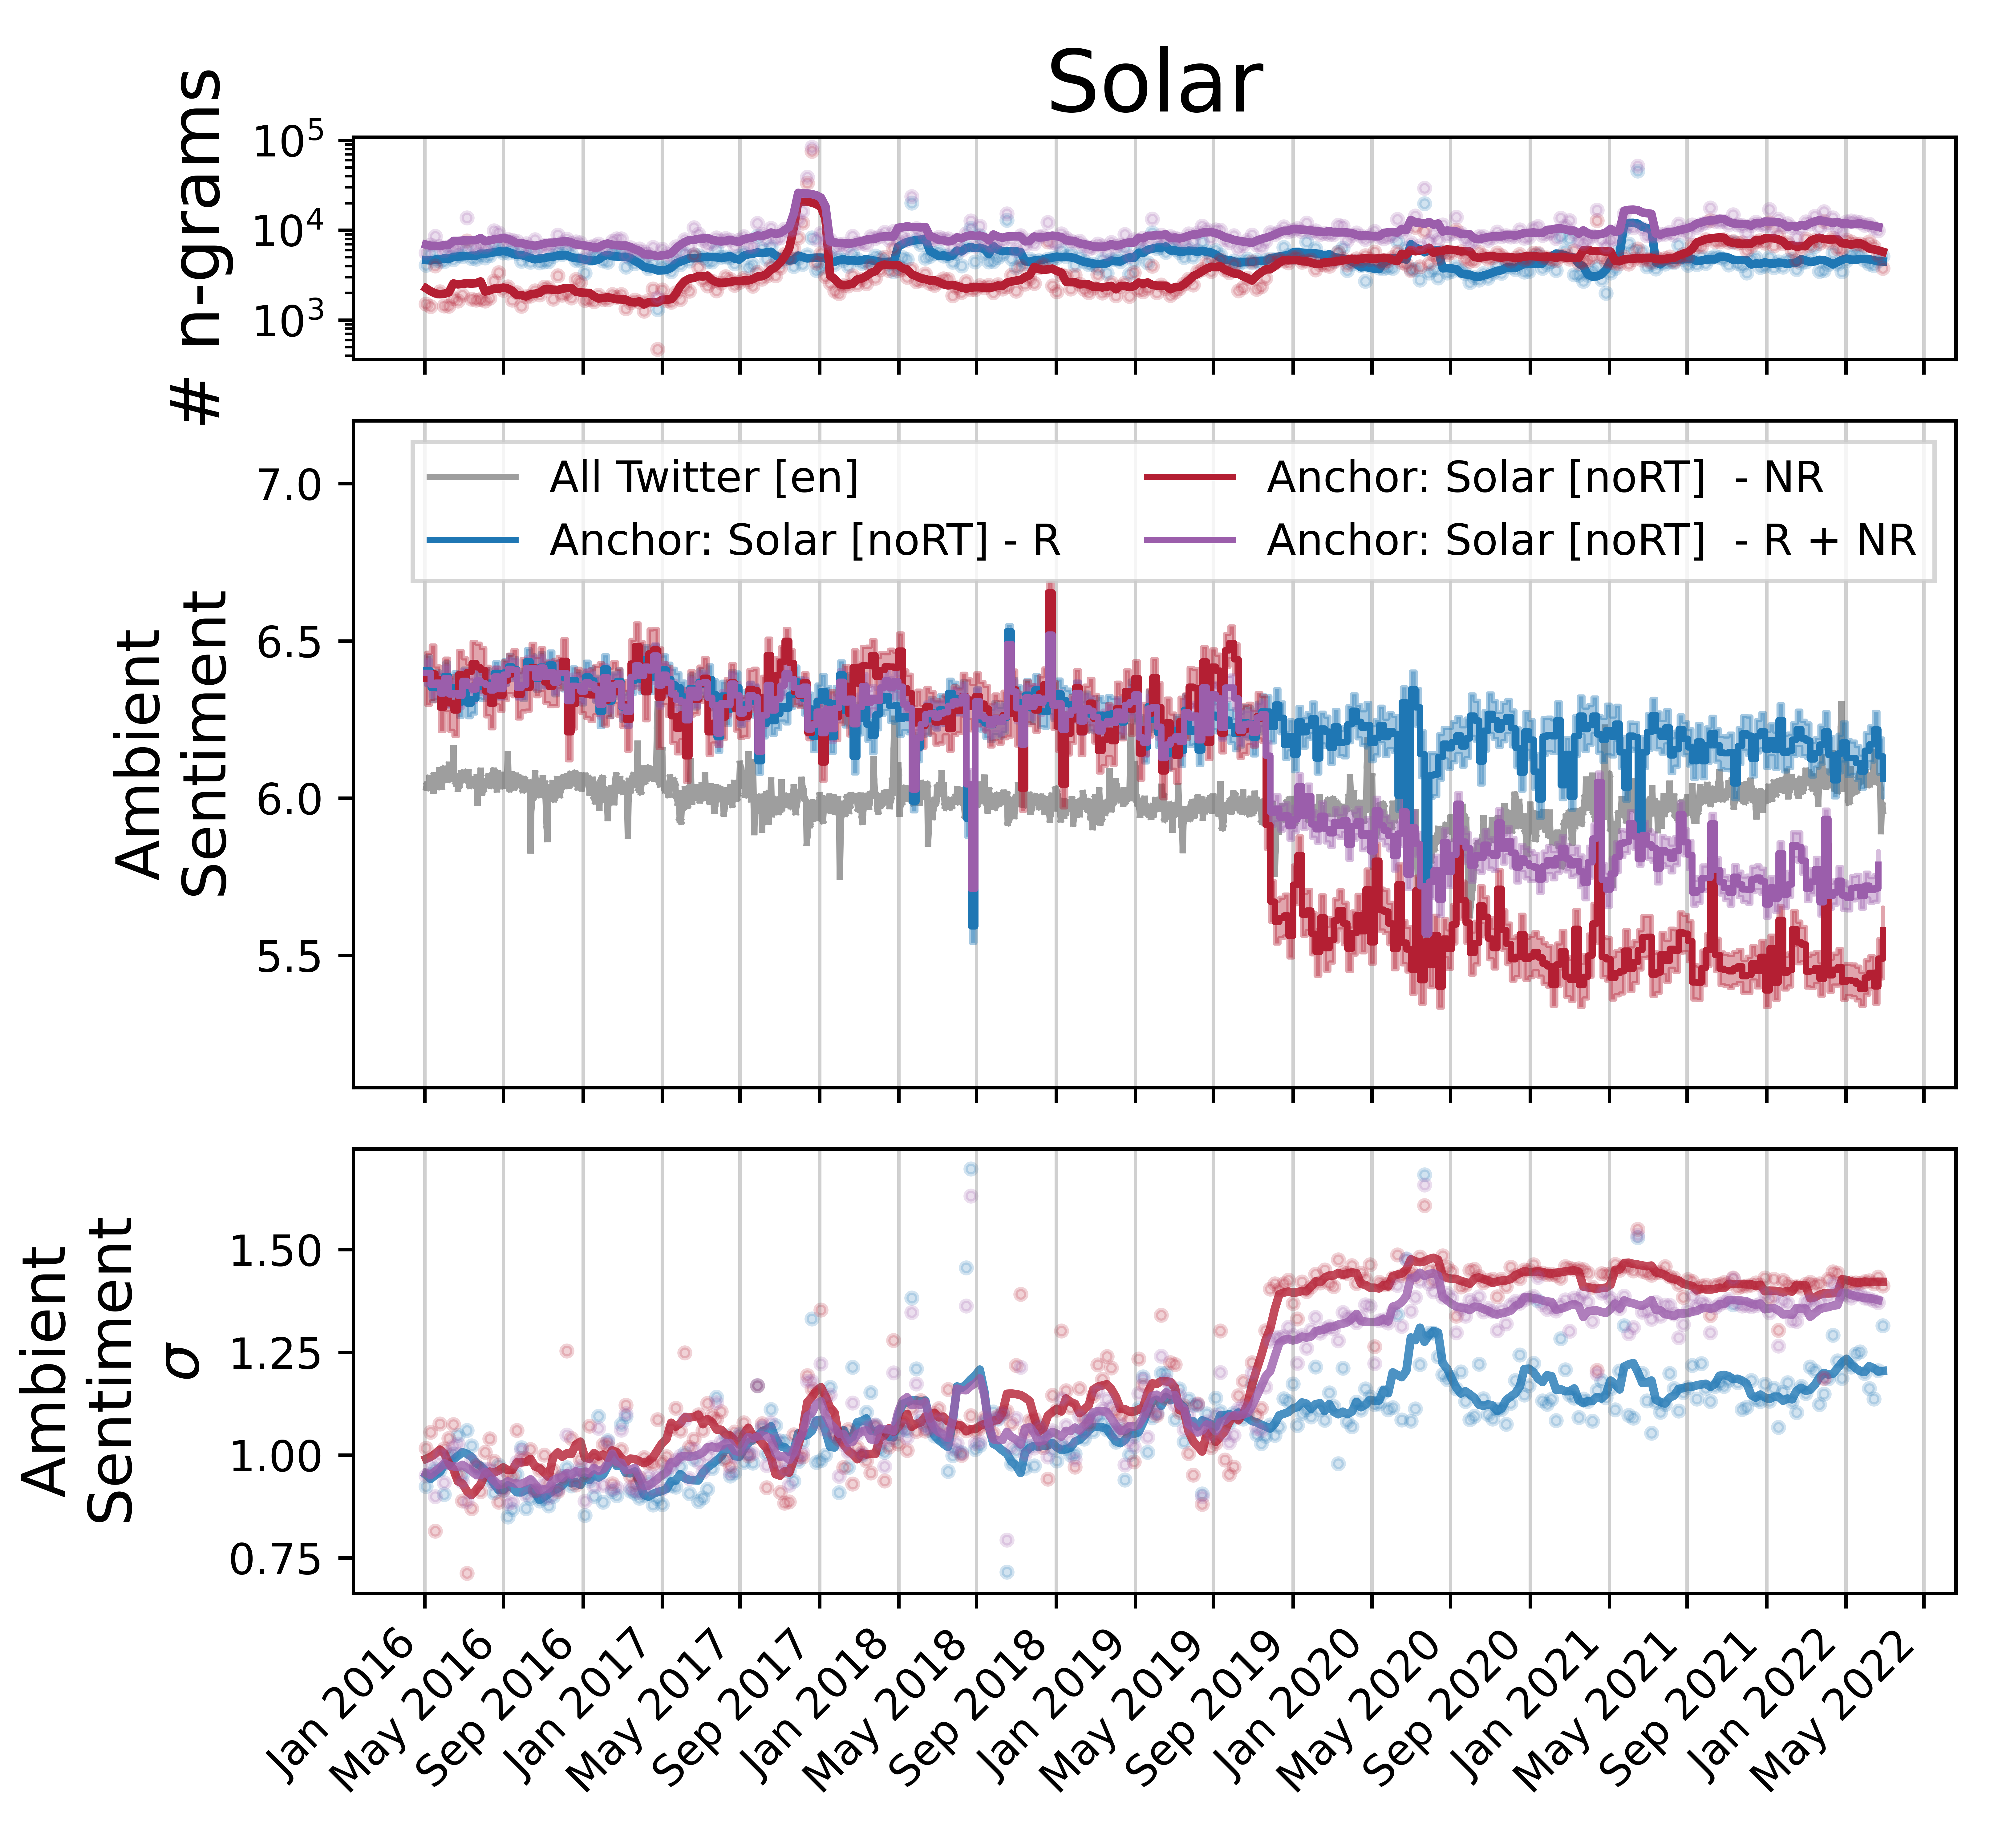
\includegraphics[width=0.98\columnwidth]{figures/Solar_sentiment_2016-01-01_2022-03-15.png}  
  \caption{
    \textbf{Ambient sentiment time series comparison for relevant  (R), non-relevant (NR), and combined tweet corpora, containing the keyword \anchor{solar}.}
    In the top panel we show the number of tokens with LabMT \cite{dodds2015human} sentiment scores in each corpus on each day.
    `Relevant' tweets, in blue, have more scored tokens early on,
    but the number tokens in `not relevant' tweets increase in relative proportion over time.
    The center panel shows the average sentiment for each corpus, including a measurement of English language tweets as a whole in gray for comparison. 
    Before 2019, the measured sentiment for both corpora are comparable, but later the mean sentiment of `non-relevant' tweets drops. 
    In the bottom panel we plot the standard deviation of the sentiment measurement, which captures a broader distribution of sentiment scores for  `non-relevant' tweets.
    Without classification filtering, the ambient sentiment measurement would been misleading, appearing as though the sentiment contained in tweets containing the word \anchor{solar} has dramatically dropped in 2019, when in fact sentiment has only modestly declined. 
  }
  \label{fig:solar_sentiment}
\end{figure}


Solar tweets were nearly evenly split with 47\% of the corpus being relevant and 53\% being not relevant by volume of words.
It also achieved the highest classification performance, achieving an F1 score of 0.95, shown in Table \ref{tab:F1-scores}.



Of the three case studies 
we found the R \anchor{solar} tweets corpus evolved
most relative to the corresponding NR corpus.
Looking at the sentiment timeseries in Fig. \ref{fig:solar_sentiment}, 
we see little difference between the ambient sentiment of the R and NR corpora prior to 2019.
Before 2019, NR ambient sentiment, shown in red, sharply falls while the R corpus appears to remain on trend.
For the standard deviation of ambient sentiment, 
which measures how broad is the distribution of sentiment scores for each LabMT word in the ambient corpus,
we also observe a dramatic increase in 2019.

We contend that the process of selecting relevant social media documents to include in a corpus
is just as important as the NLP measurement tools
used to quantify sentiment.
The difference in resulting sentiment measurements,
between what would have been measured without a classifier
(the R + NR corpus in purple) 
and the improved measurement after filtering with a classifier 
(the R corpus in blue) 
is stark. 
Looking at only the combined R + NR measurement,
researchers could incorrectly conclude that language surrounding \anchor{solar}
has decreased in sentiment dramatically since 2019. 

Focusing on only the R \anchor{solar} sentiment timeseries,
it is clear that there was no dramatic drop in sentiment around \anchor{solar}, 
and this language remains more positive relative to English language tweets in general. 
The decrease in observed NR sentiment is likely related to an influx of weather bots,  
which provide updates as often as hourly on local weather conditions
and contain \anchor{solar} used in the context of measuring current solar radiation. 
In Fig. \ref{fig:combined_sentiment_shifts} we see terms like `radiation', `pressure', and `humidity' are contributing to a lower average sentiment for the NR corpus.

Examining Fig. \ref{fig:rankdiv_solar} we can see terms like `energy', `power', and `panels' are much more common in the R corpus, all being among the top 15 most frequently used terms. Weather related terms like `mph', `uv', `radiation', and `gust' are top words in the non-relevant corpus. 

\todo{worried about redundancy with the figure caption}

\todo{wrap-up for solar, what did we learn, }



\subsection{Wind Energy Case Study}

\begin{figure}[tp!]
  \centering	
    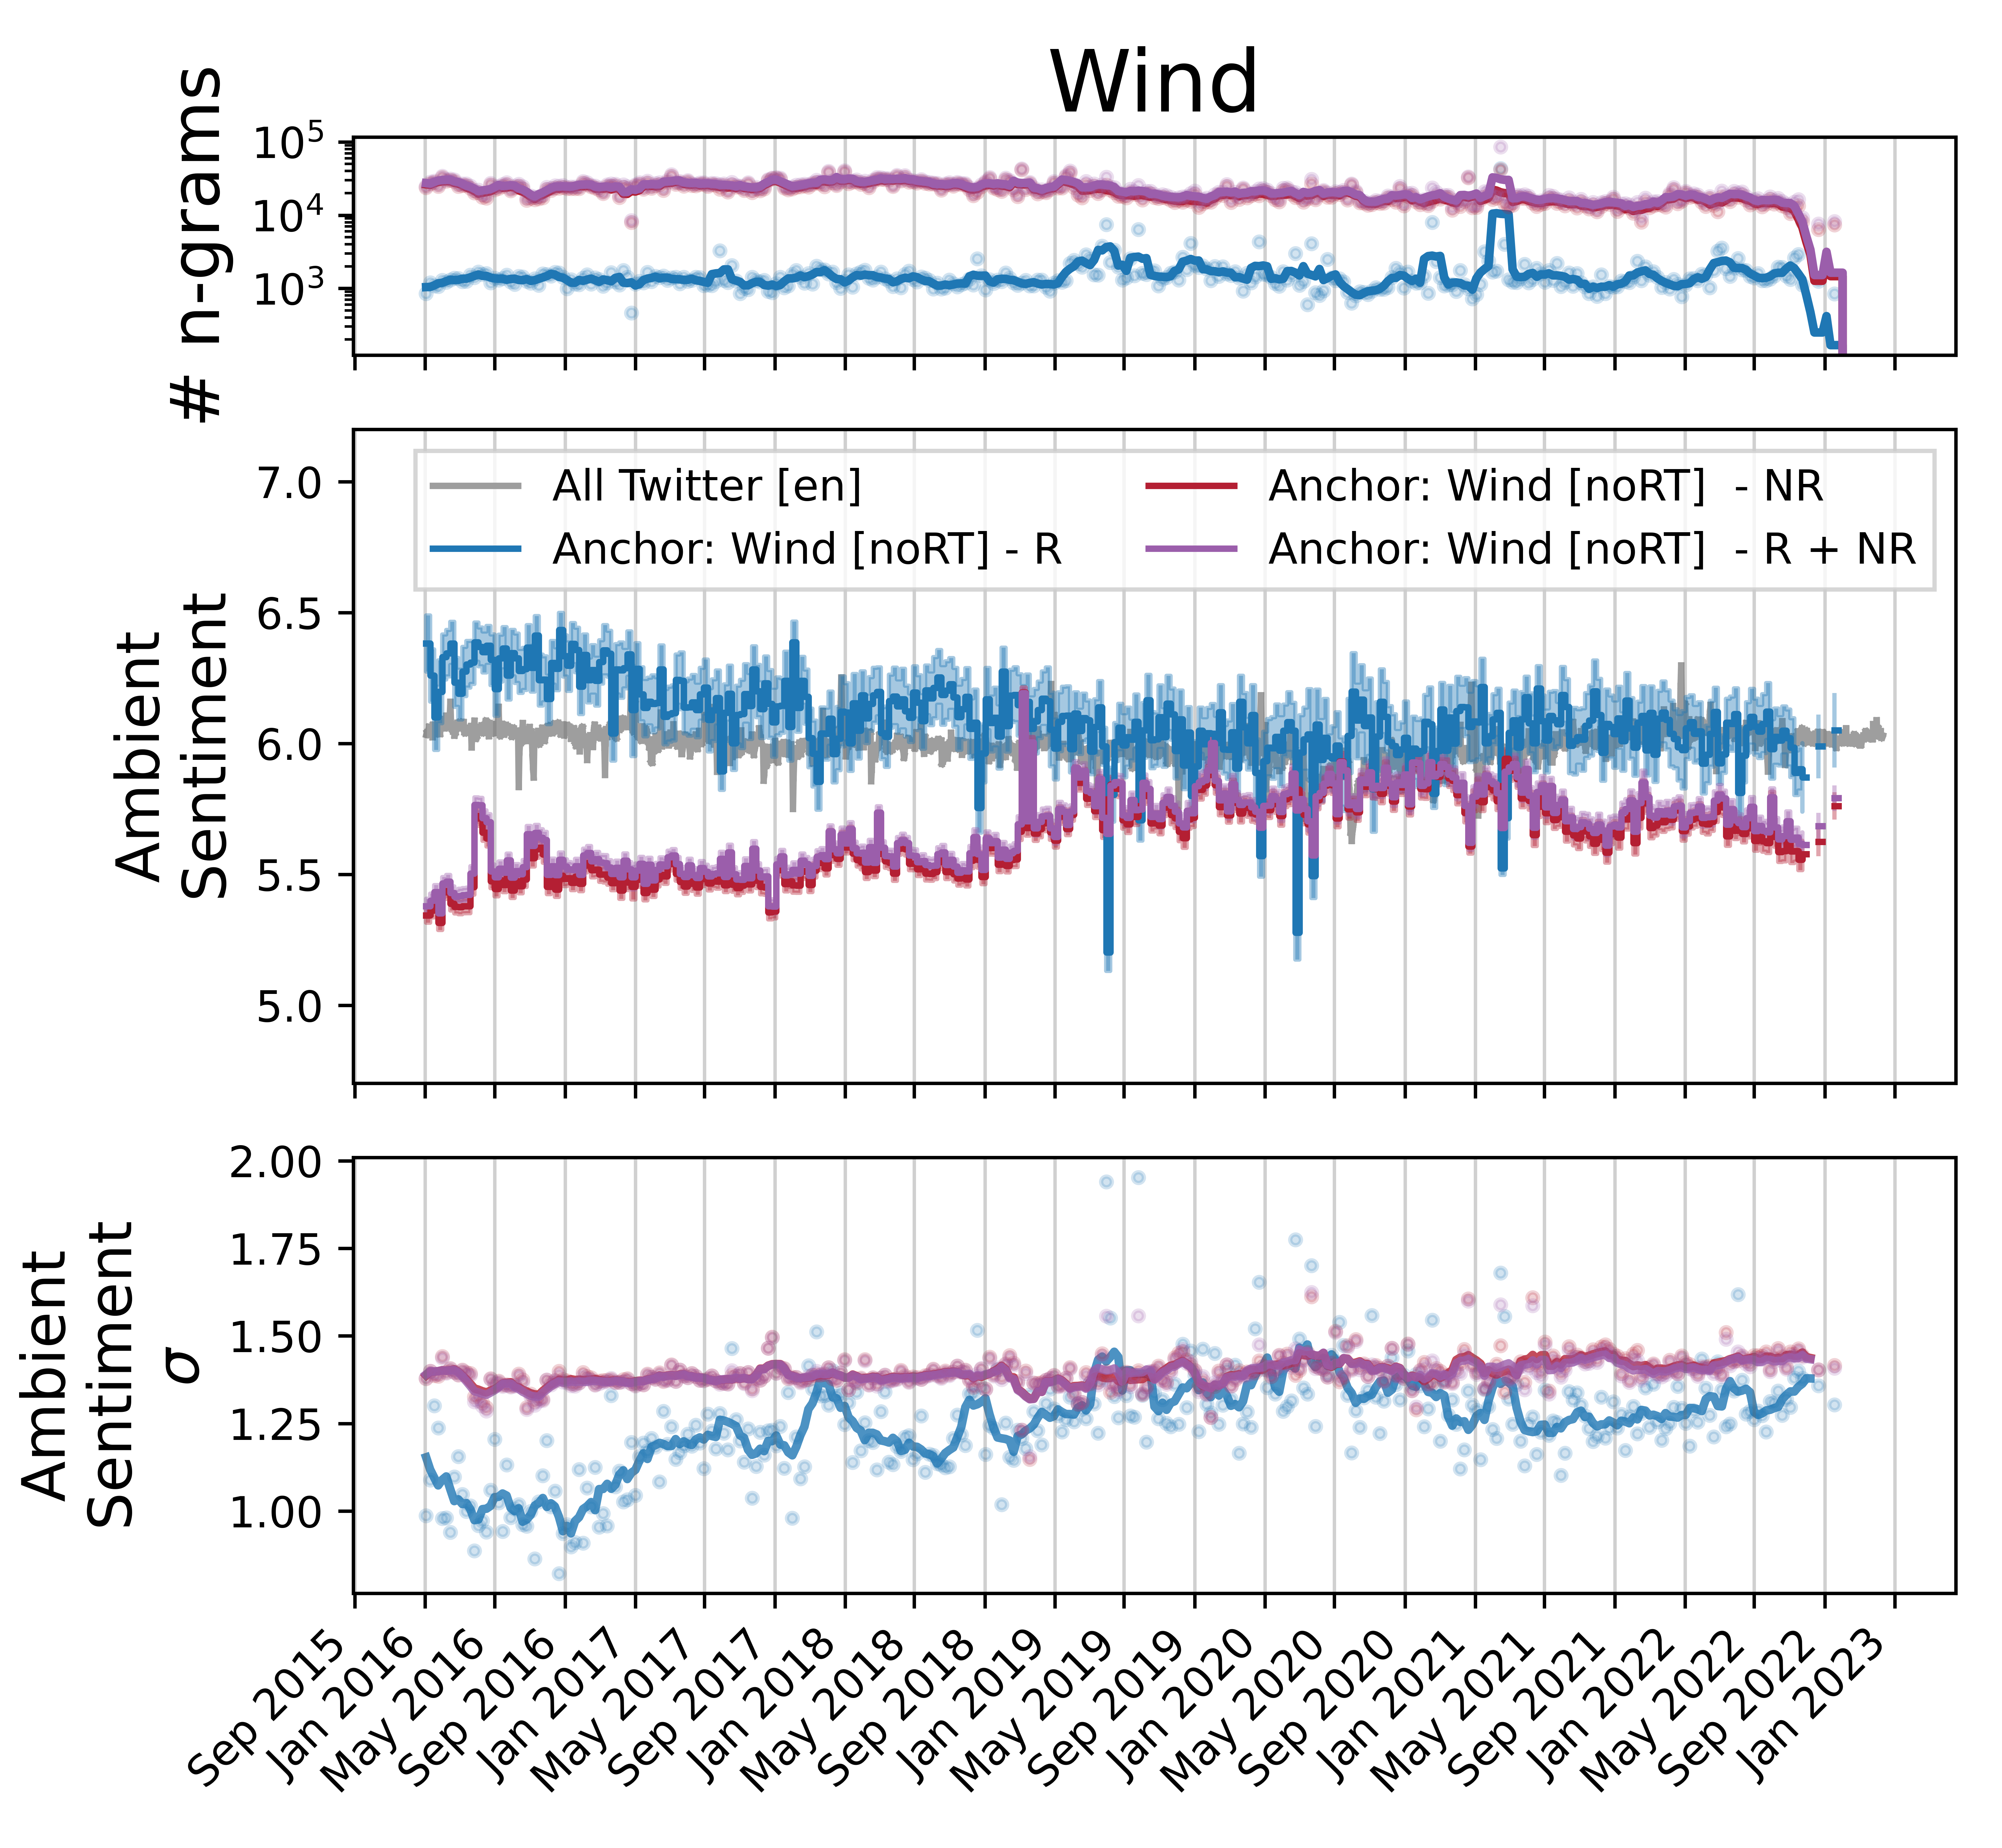
\includegraphics[width=0.98\columnwidth]{figures/Wind_sentiment_2016-01-01_2022-08-30.png}  
  \caption{
    \textbf{Ambient sentiment time series comparison for relevant  (R),
    non-relevant (NR), and combined tweet corpora,
    all containing the keyword \anchor{wind}.}
    In the top panel we show the number of tokens with LabMT
    sentiment scores for each corpus on each two week period~\cite{dodds2015human}.
    R tweets, in blue, have more than an order of magnitude fewer tokens per time window over the entire study period.
    The center panel shows the average sentiment for each corpus, including measurement of English language tweets as a whole in gray for comparison. 
    R \anchor{wind} tweets are more positive than Twitter on average early on, but this difference is reduced over time. 
    Because most \anchor{wind} tweets are not relevant, both the sentiment of the combined corpus closely follows the NR sentiment.
    In the bottom panel we plot the standard deviation of the sentiment measurement,
    which captures a broader distribution of sentiment scores for  `non-relevant' tweets,
    as was the case for all case-studies we examined.
    Without classification filtering, the ambient sentiment measurement would have been dominated by NR tweets. 
  }
  \label{fig:wind_sentiment}
\end{figure}
\todo{}
The unclassified \anchor{wind} tweets corpus had the lowest proportion of relevant tweets;
only 5\% of the human labeled subset was related to clean energy.
The n-gram \anchor{wind} is used in many different contexts besides energy generation,
from casual discussion of today's weather to figurative uses like references to athletes getting their `second wind' and the anticipatory rotational phrase `wind up' where `wind' rhymes with `kind'. In the top panel of Figure \ref{fig:wind_sentiment}, we can see that the number of n-grams in relevant tweets with corresponding sentiment scores is consistently around $10^3$, while the NR corpus contain more than an order of magnitude more text.

We found the ambient sentiment of the R \anchor{wind} corpus has been slightly more positive than average language use on Twitter. 
The NR corpus had distinctly lower sentiment, but was more dynamic, rising from a low of 5.5 in 2016, to 5.9 in 2020.
Because the proportion of tweets relevant to energy is so low, 
the combined sentiment time series measurement is dominated by the NR corpus. 
The standard deviation of sentiment, $\sigma$, for the R corpus also increased from around 1.0 in 2016, before leveling off around 1.2, slightly under the NR corpus.




The choice of \anchor{wind} could seem to be an irresponsible choice of keyword, 
given that the vast majority of matching tweets are not relevant.  
Under a paradigm  of expert-crafted lists of keywords, we would agree it isn't suitable. 
However, by choosing such a potentially ambiguous term, we're able to capture a wider range of users. 
Those who don't wish to project their thoughts into a global conversation by attaching a hashtag, but are content with discussing among their local network are still included with this methodology. 
Also included are users writing informally or using context of a threaded conversation, who might not use a high precision keyword phrase, like `wind power', `wind generation', or `wind energy'.
These cases make up a significant proportion of conversation around any given topic; researchers studying more obscure topics could benefit from the increased sample size, and temporal resolution of a higher recall set of keywords.

\subsection{ Nuclear Energy Case Study}

\begin{figure}[tp!]
  \centering	
    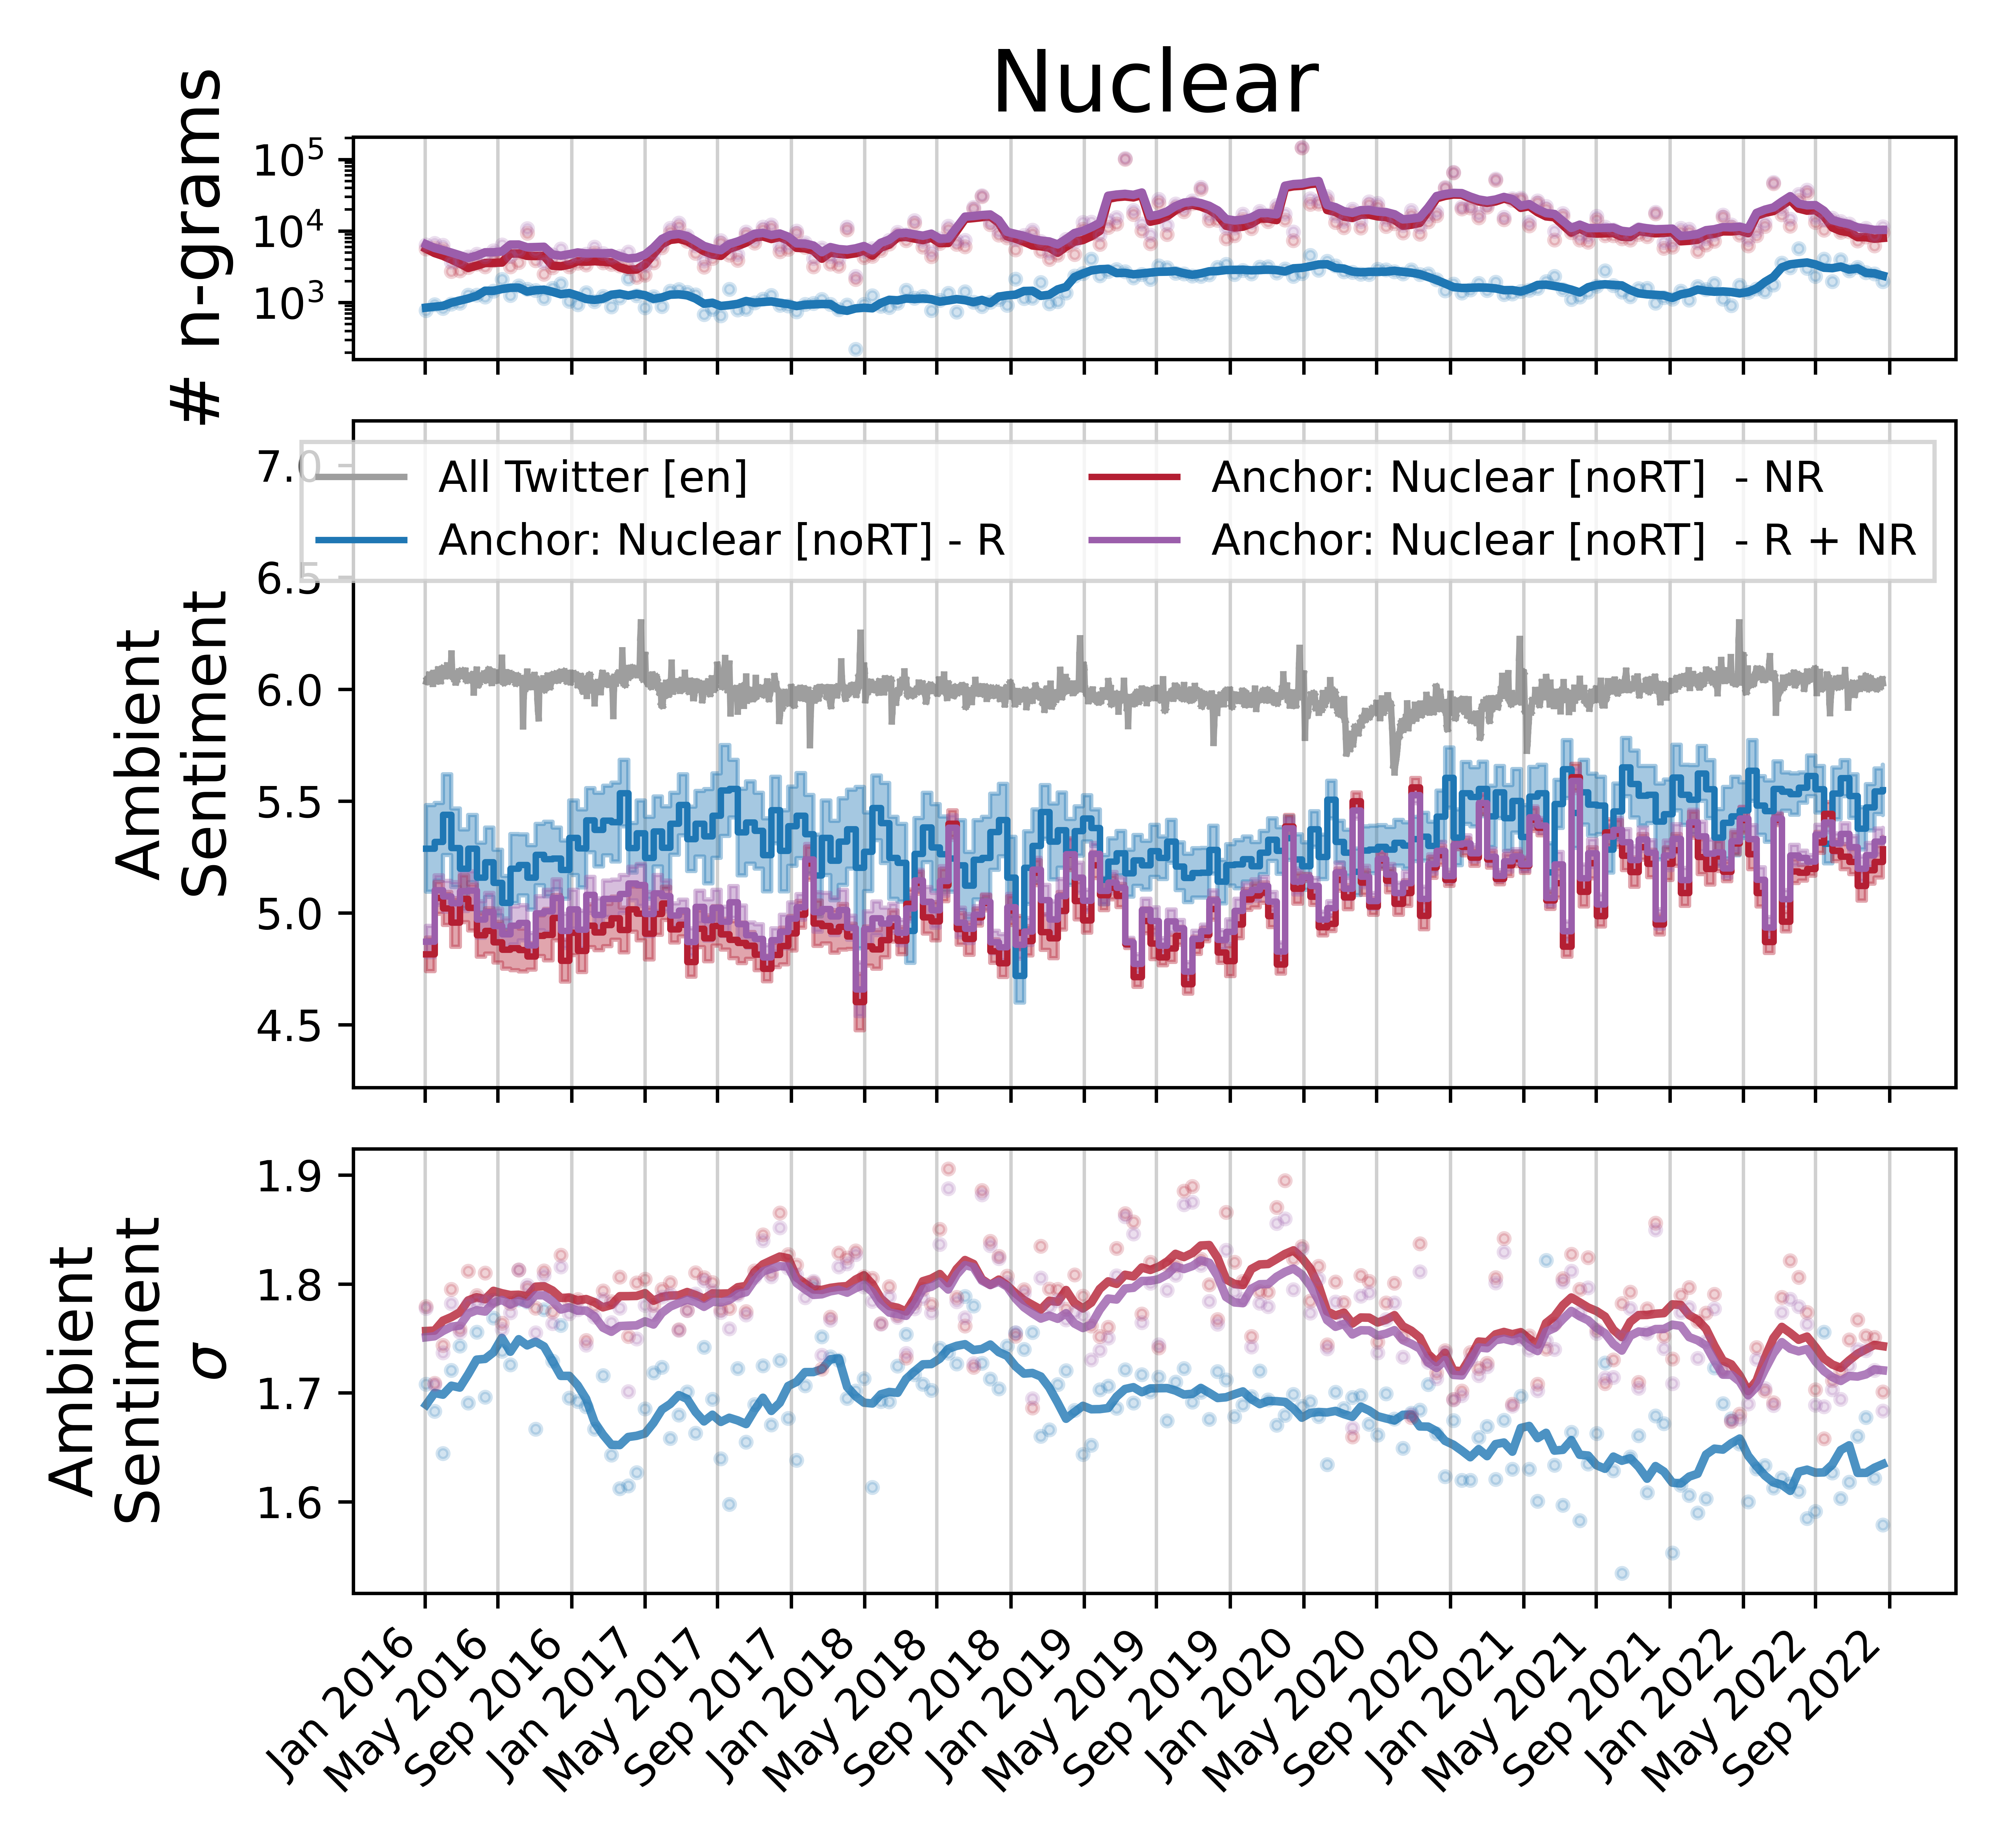
\includegraphics[width=0.98\columnwidth]{figures/Nuclear_sentiment_2016-01-01_2022-08-31.png}  
  \caption{
    \textbf{Ambient sentiment time series comparison for relevant (R), non-relevant (NR), and combined tweet corpora,
    all containing the keyword \anchor{nuclear}.}
    In the top panel
    we show the number of tokens with LabMT \cite{dodds2015human}
    sentiment scores for each corpus in each two week period.
    The number of relevant n-grams,
    in blue,
    is consistently lower than non-relevant n-grams. 
    The center panel shows the average sentiment for each corpus,
    including measurement of English language tweets as a whole in gray. 
    We found that
    R tweets had higher sentiment than NR tweets
    containing \anchor{nuclear},
    but had much lower sentiment than Twitter as a whole.
    Sentiment appears relatively stable for both corpora
    with periods of higher sentiment around 2017 and 2020-2022 for the R corpus.
    In the bottom panel we plot the standard deviation of the sentiment measurement, which shows a broader distribution of sentiment scores for NR tweets and both corpora trending down slightly. 
  }
  \label{fig:nuclear_sentiment}
\end{figure}

The \anchor{nuclear} case study had the lowest classification performance after fine-tuning, 
achieving an F1 score of just 0.86. 
The proportion of relevant tweets, 16\%, was higher than for the \anchor{wind} corpus. 
We believe the performance was impacted negatively by the close proximity and overlap
of nuclear energy and nuclear weapons topics in the semantic embedding space. 

% nuclear sentiment
The ambient sentiment timeseries, in Fig. \ref{fig:nuclear_sentiment},
for the R \anchor{nuclear} corpus was much lower than average sentiment on Twitter for the entire study period,
but higher than the NR corpus.
It appears that ambient sentiment around R nuclear energy tweets has been increasing, with a higher stable level since fall 2020. 
We found that the standard deviation of sentiment is also decreasing slightly,
though it starts from a much higher level of around 1.7, compared to less controversial technologies, wind and solar.

% nuclear sentiment shift
In Fig. \ref{fig:combined_sentiment_shifts} we can see that this difference in sentiment is driven by more positive words in the relevant corpus,
like `power' and `energy',
but also fewer negative words,
like `war' and `weapons', relative to the NR corpus.
`Waste' is a negatively scored word that used much more frequently in the R corpus relative to the NR corpus.




\begin{figure*}
  \centering	
    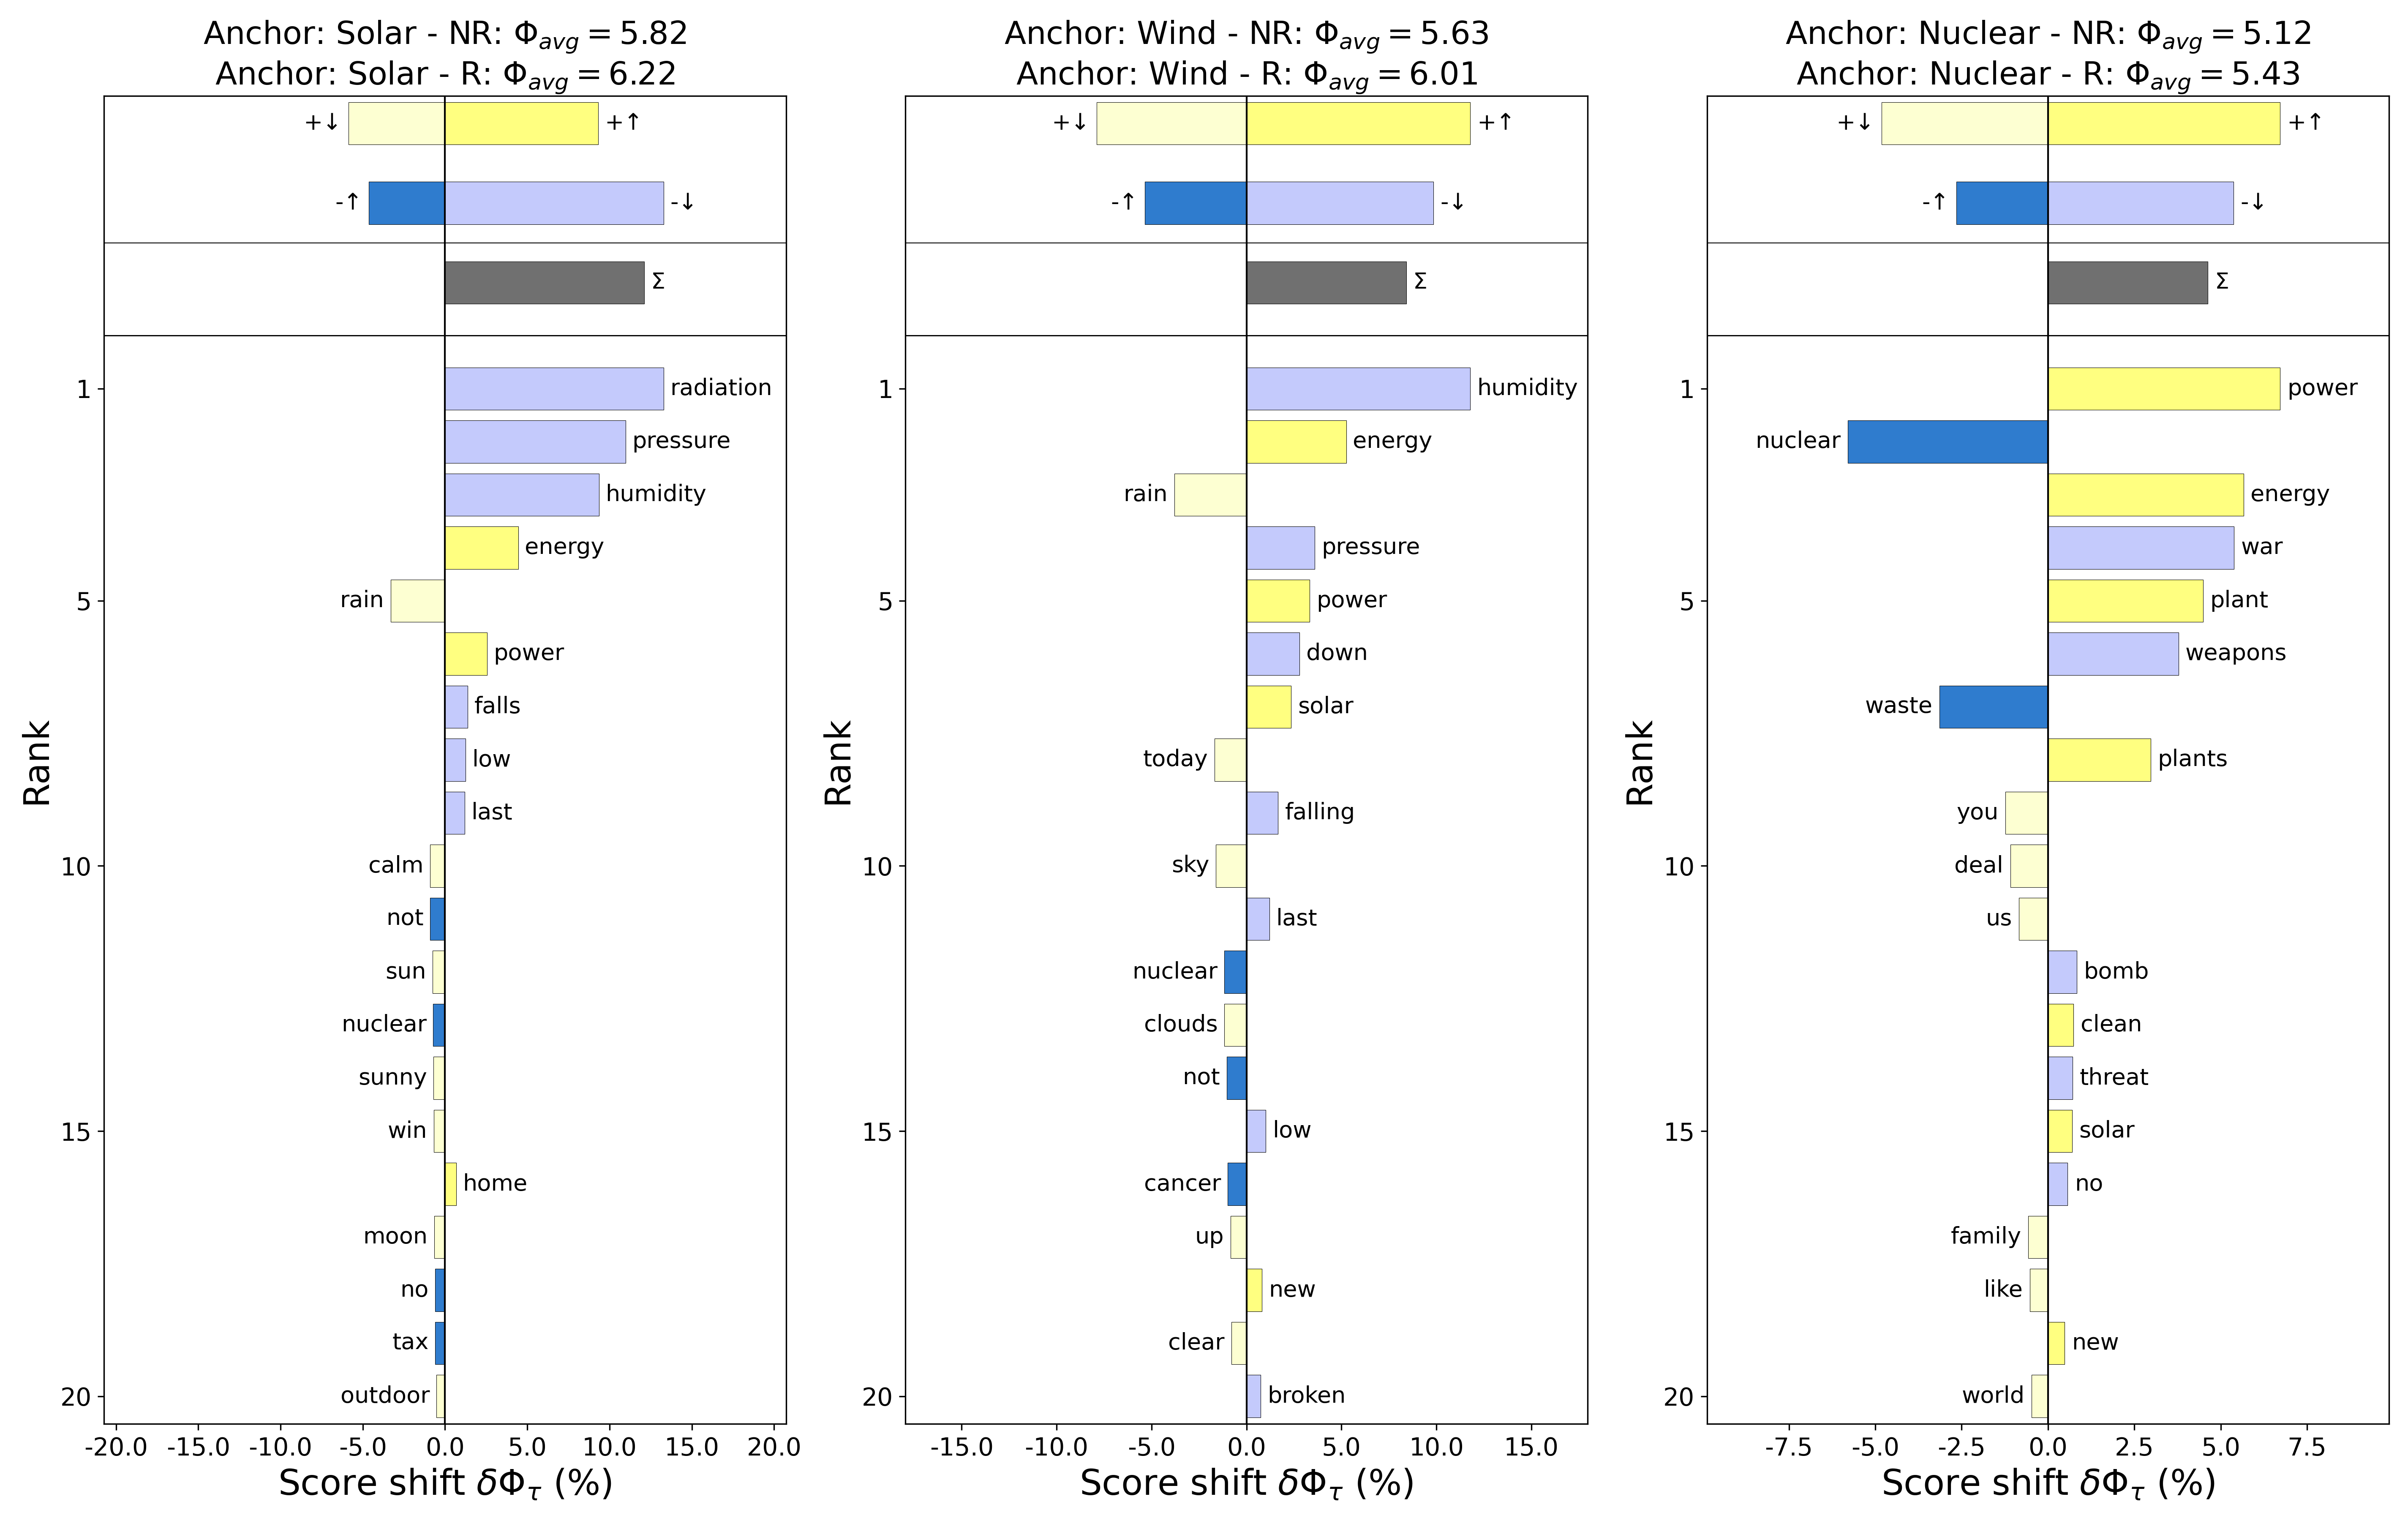
\includegraphics[width=0.98\textwidth]{figures/combined_shifts.png}  
  \caption{
    \textbf{Sentiment shift plots comparing the classified `relevant' (R) and `non-relevant' (NR) tweet corpora for tweets containing the keywords \anchor{solar}, \anchor{wind}, and \anchor{nuclear}.}
    We show the 20 top contributing words to the difference in LabMT sentiment between the corpora.
    `Relevant' tweets, those related to clean energy
    are more positive on average for all keywords
    when compared to `not relevant' tweets. 
    Sad words that are less common in `relevant' \anchor{solar} tweets are `radiation', `pressure', and `humidity', which largely refer to the weather.
    Happy words like `energy' and `power' are more common in `relevant' tweets compared to tweets not relevant to solar energy. For \anchor{wind} sad terms like `humidity' and `pressure' are less common in `relevant' tweets,
    while happy terms like `energy', `power', and `solar' are more common in tweets relevant to wind as a renewable energy source. 
    For \anchor{nuclear}, relevant tweets are on average more positive due to sad words like `war', `weapons', and `bomb' being less common in relevant tweets,
    while happy words like `power' and `energy' are more common.
    Some sad words like `nuclear' and `waste' do occur more frequently in relevant tweets.
  }    
  \label{fig:combined_sentiment_shifts}
\end{figure*}


\begin{figure*}
  \centering	
    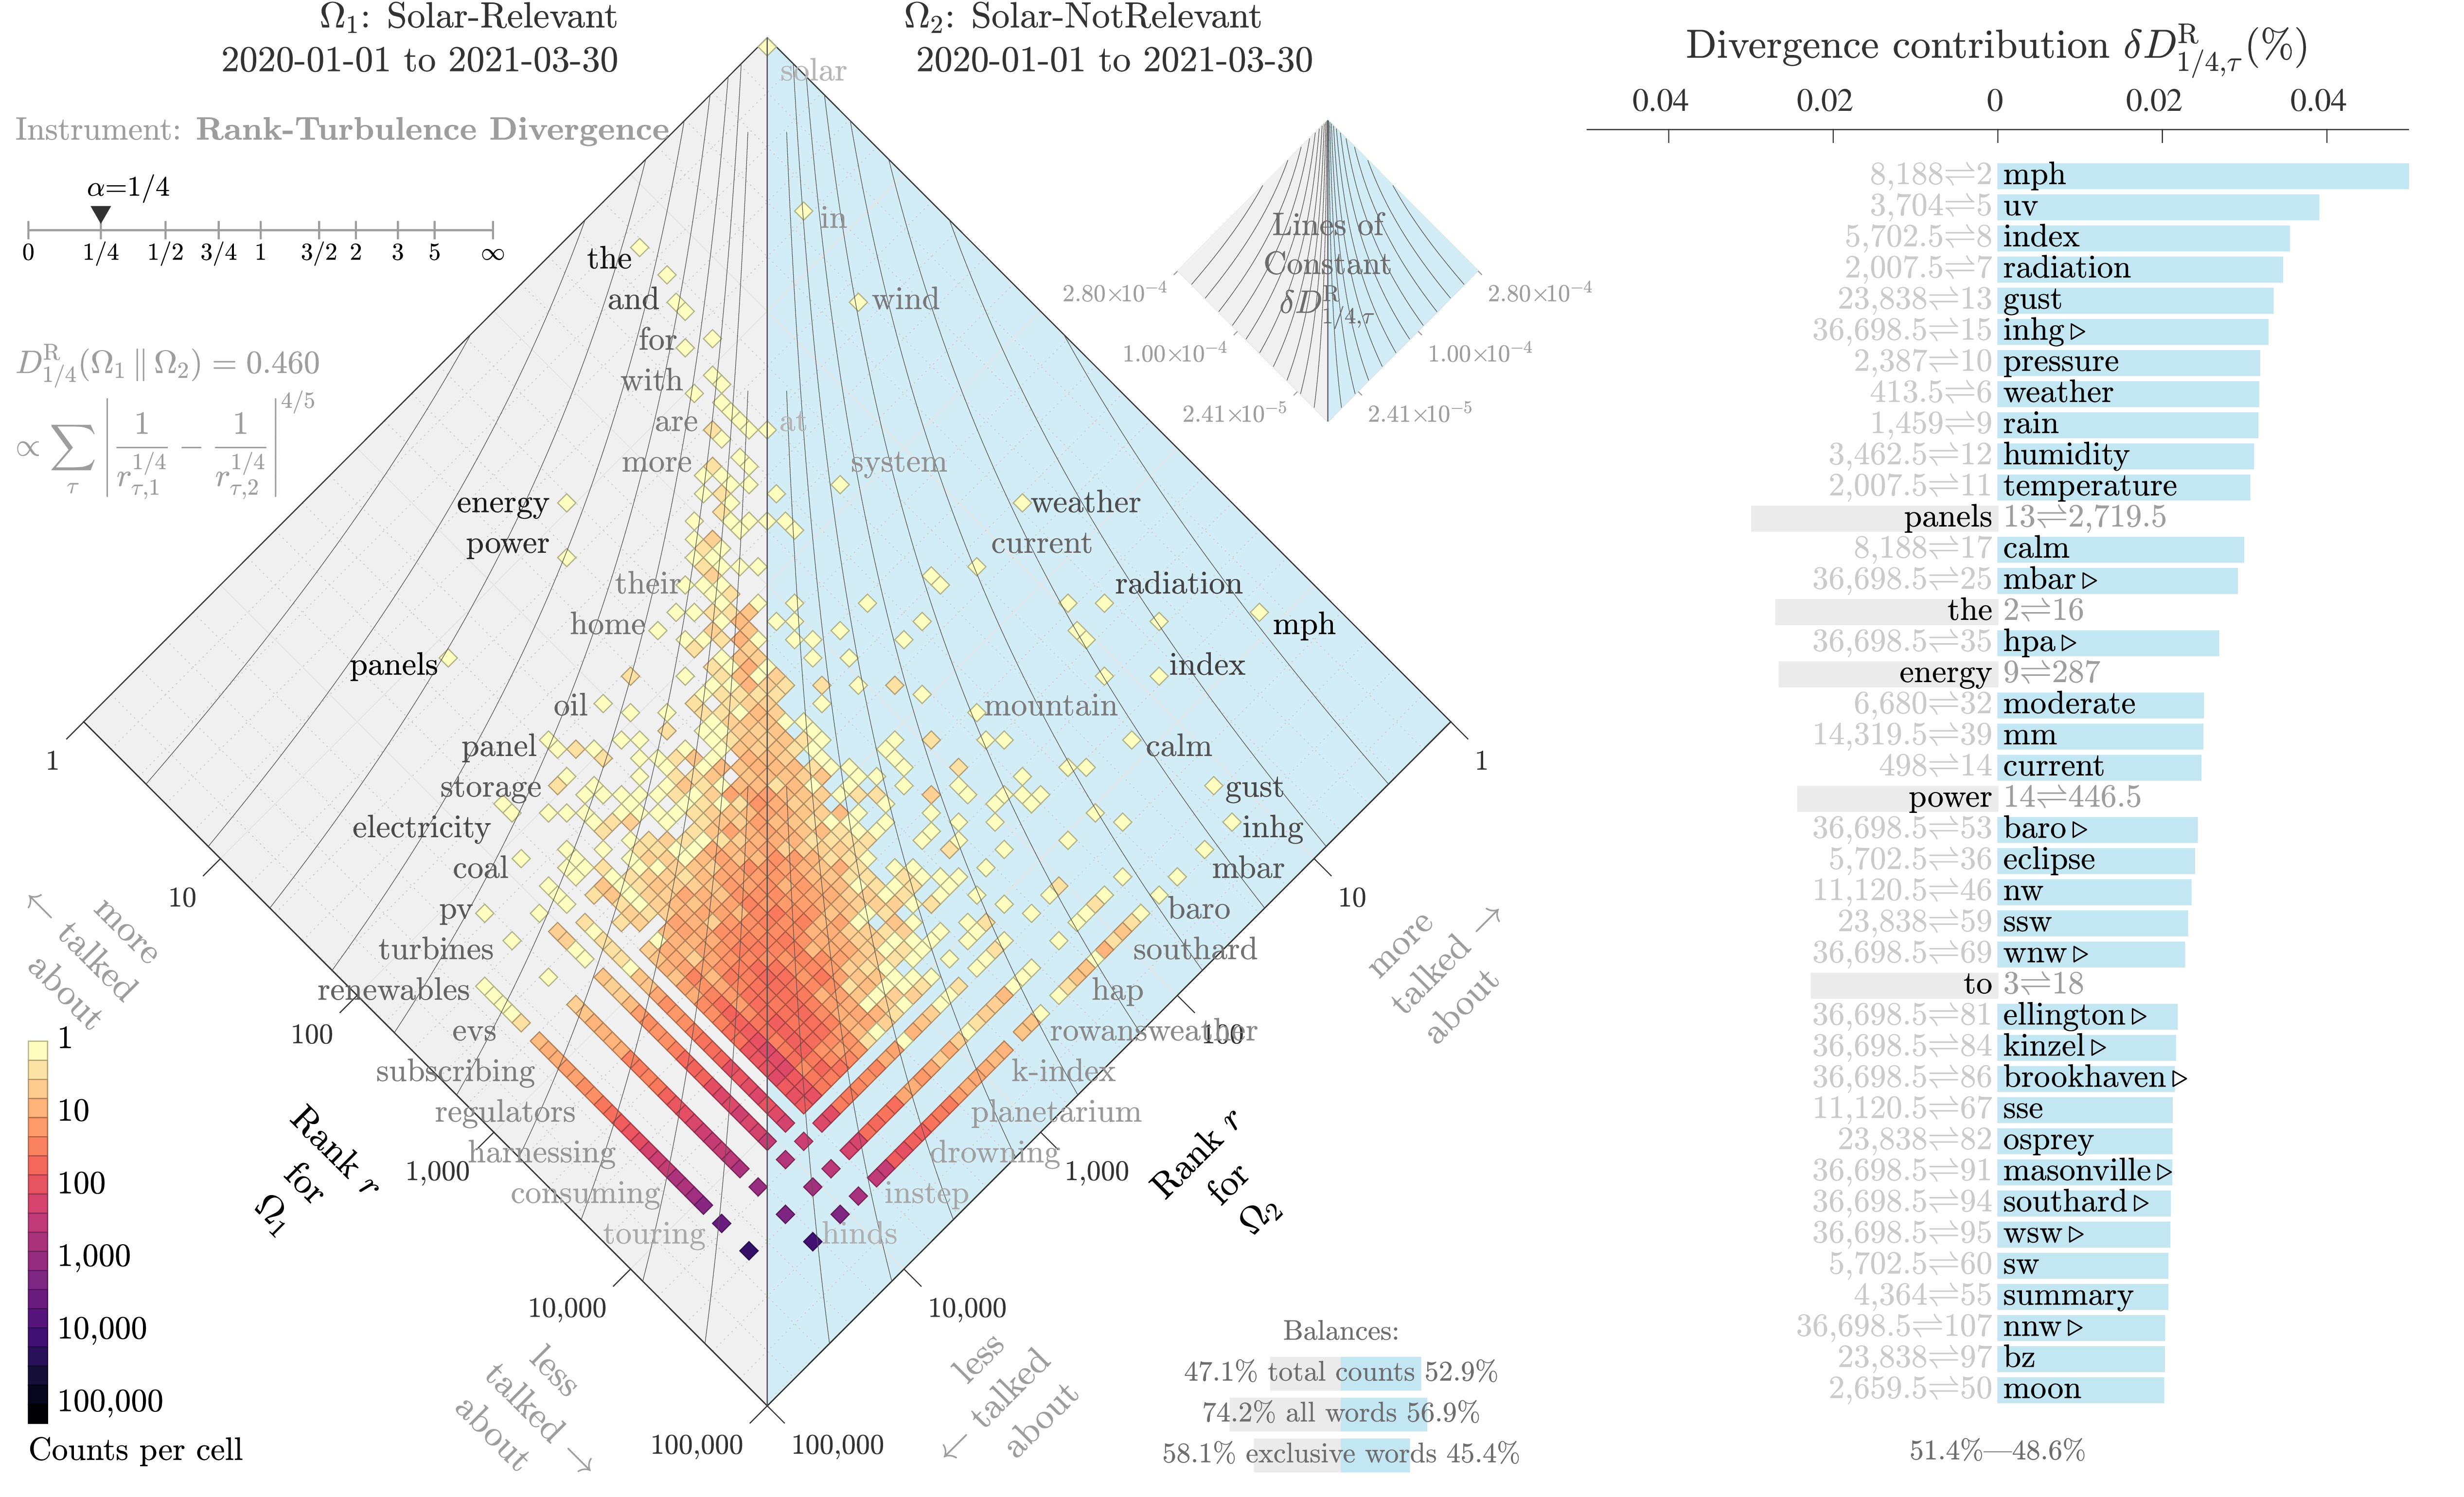
\includegraphics[width=0.90\textwidth]{figures/figallotaxonometer9000-2021-03-30-2021-03-30-rank-div-alpha-third-Solar_Solar_noname.png}  
  \caption{\textbf{Allotaxonograph comparing the rank divergence of words
    classified as relevant to solar energy discourse
    to those containing the keyword \anchor{solar}
    but classified as not relevant.} 
    On the main 2D rank-rank histogram panel,
    words appearing on the right have a higher rank in the ``relevant'' subset than in ``not relevant'', while phrases on the left appeared more frequently in the ``not relevant'' tweets.
    The panel on the right shows the words which contribute most to the rank divergence between each corpus.
    %% examples
    We observe that many words associated with weather bots,
    such as ``mph,'' ``uv,'' and ``pressure,'' 
    are more frequently used in non-relevant posts,
    while words like ``panels,'' ``energy,'' and ``power,'' used more in tweets relevant to solar energy.
    Notably, commonly used function words,
    such as ``the,'' ``and,'' and ``are,'' 
    are off-center in the rank-rank histogram, a further indication that many of the ``not relevant'' tweets are from automated accounts publishing weather data rather than using conversational English.
    The balance of the words in these two subsets is noted in the bottom right corner of the histogram, showing the percentage of total counts, all words, and exclusive words. 
    For this example the two subsets are nearly balanced, indicating that the filtered corpus contains less than 50\% of word tokens from the raw query.
    See Dodds~\etal~\cite{dodds2020allotaxonometry} for a full description of the allotaxonometric instrument.}
    \label{fig:rankdiv_solar}
\end{figure*}


\section{Concluding remarks}
\label{sec:corpusCreation.concludingremarks}


\todo{limitations, not a representative sample, etc}

We hope this work can highlight
an alternative corpus curation framework
for computational social scientists. 
Rather than defining the boundaries of a corpus by a set of expert defined rules,
researchers can look at a sample of data, 
label messages as relevant as they see see fit,
and communicate their reasoning directly,
along with the set of released data.

We have demonstrated that text classifiers can be trained on top of pre-trained contextual sentence embeddings,
which can accurately encode researcher discretion
and infer the relevance of millions of messages on a laptop. %more here




Future work could explore better sampling methods for humans labeling tweets
to reduce the amount of labeled data needed to train the text classifier. 
Sampling messages by shuffling
risks oversampling
from dense regions of the semantic embedding space. 
The coder sees repetitive messages that provide little marginal 
information to the model.
This would have negative impacts on the generalizability of the classifier, and we would be skeptical of real-time measurements as conversation could drift into under-explored regions of the semantic embedding space.
Other work could explore the trade-offs between optimizing for high recall and high precision when curating  social media datasets, and the impacts on resulting measurements. 

For online applications of relevance classifiers, such work would be useful in identifying when more training data is needed. 
By measuring changes in language use, both by measuring rank-turbulence divergence ~\cite{dodds2020allotaxonometry}
or Jensen–Shannon divergence~\cite{dhillon2003divisive} between the training corpus and incoming data,
and by measuring changes in the distribution of messages within a semantic embedding, thresholds for train data updates could be determined.

Finally, researchers could explore viewing social media datasets as having uncertain boundaries, 
and running measurements over data set ensembles
to better capture the uncertainly in researcher discretion inherent in corpus curation.